%%%%%%%%%%%%%%%%%%%%%%%%%%%%%%%%%%%%%%%%%%%%%%%%%%%%%%%%%%%%%%%%%%%%%%%%%%%%%%
\section{DAQ configuration}

The system supports multiple run configurations, as shown in Figure~\ref{figure:run_configurations}

\begin{itemize}
\item 
  Run configurations are stored in the "/Mu2e/RunConfigurations" subtree
\item
  each run configuration is an independent subtree, any modification
  of a given run configuration doesn't affect other run configurations
\item
  a run configuration template can be saved as a .json structure and loaded from
  an external .json file, for example
\begin{verbatim}
mu2etrk@mu2edaq22:~/test_stand/pasha_031>odbedit
[local:test_025:S]/>cd Mu2e/Run
[local:test_025:S]/>cd Mu2e/RunConfigurations/demo
[local:test_025:S]demo>save demo.json
[local:test_025:S]demo>exit
\end{verbatim}
\item
  ODB links are allowed, but have to point within the configuration
\item
  configuration templates are archived on github. 
\end{itemize}

\begin{figure}[H]
  \begin{tikzpicture}
    \node[anchor=south west,inner sep=0] at (0,0.) {
      % \node[shift={(0 cm,0.cm)},inner sep=0,rotate={90}] at (0,0) {}
      \makebox[\textwidth][c] {
        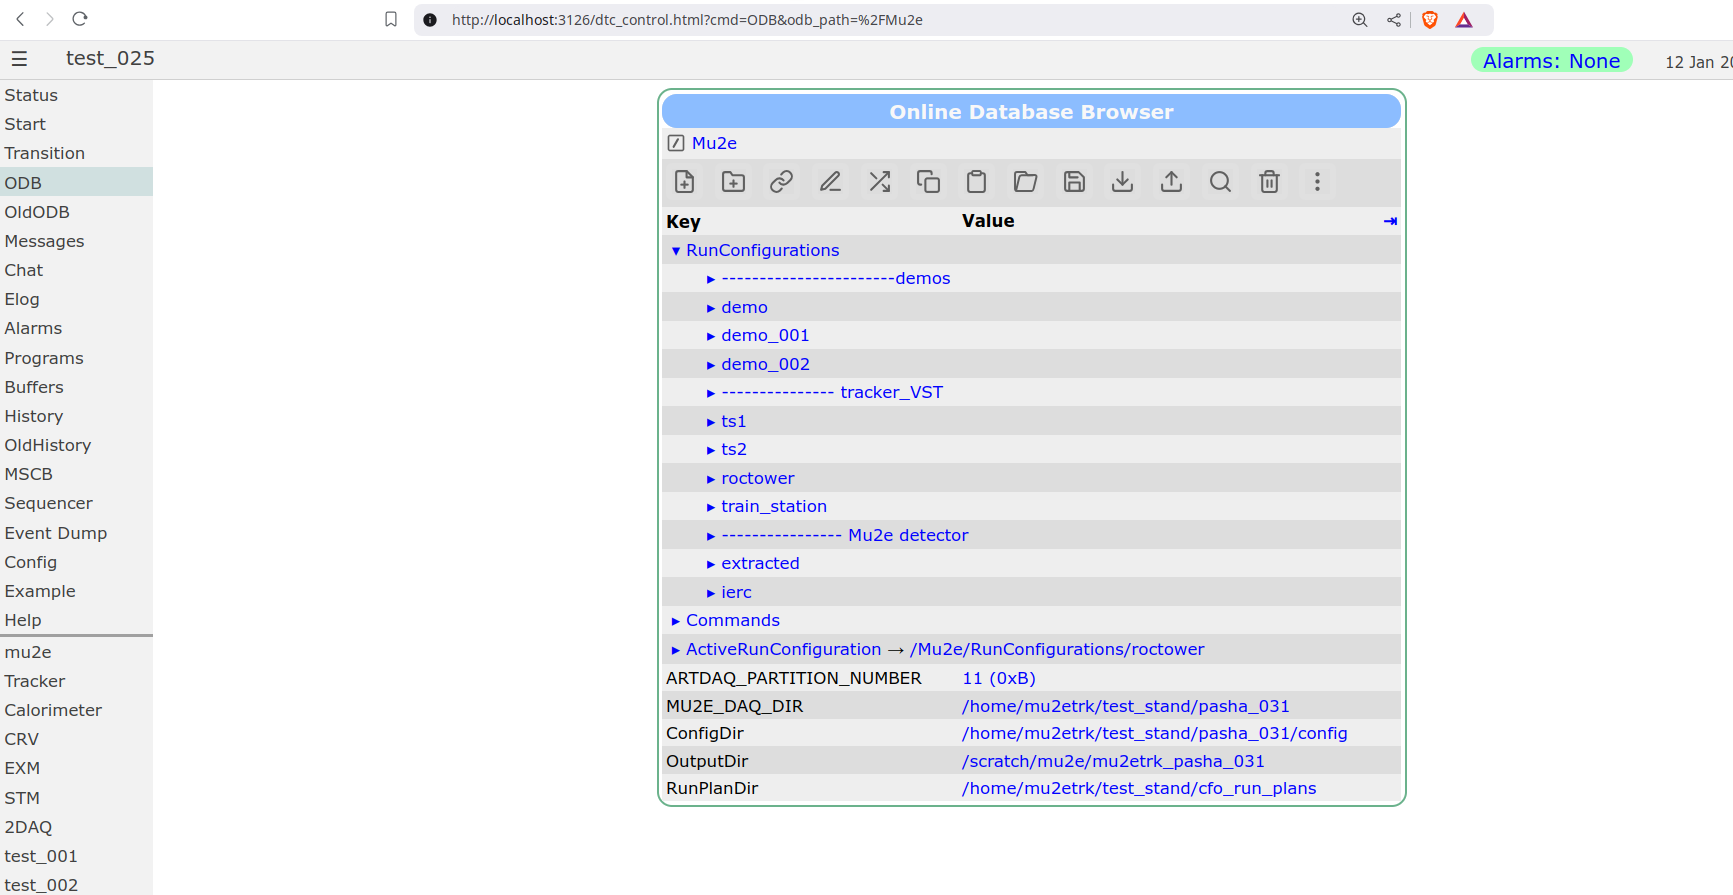
\includegraphics[width=0.95\textwidth]{png/run_configurations}
      }
    };
    % \node [text width=8cm, scale=1.0] at (14.5,0.5) {$\mu_B$, expected background mean};
    % \node [text width=8cm, scale=1.0, rotate={90}] at (1.5,7.5) { $S_{D}$, ``discovery'' signal strength  };
  \end{tikzpicture}
  \caption{
    \label{figure:run_configurations}
    Top-level run configurations
  }
\end{figure}

\begin{itemize}
\item 
  a configuration has a name, a status, and a list of subdetector configurations,
  as shown in Figure~\ref{figure:configuration_top}
\item
  each subdetector has a separate configuration subtree
\item
  templates for the subdetector configurations are stored in the 
  \href{https://github.com/pavel1murat/frontends/tree/main/odb/Mu2e/Subdetectors}
  {\blue frontends/odb/Mu2e/Subdetectors} subdirectory
\item
  Shown in  Figure~\ref{figure:run_configurations} ODB element "/Mu2e/ActiveRunConfiguration" is an ODB link
  pointing to the currently active configuration.
\end{itemize}

\begin{figure}[H]
  \begin{tikzpicture}
    \node[anchor=south west,inner sep=0] at (0,0.) {
      % \node[shift={(0 cm,0.cm)},inner sep=0,rotate={90}] at (0,0) {}
      \makebox[\textwidth][c] {
        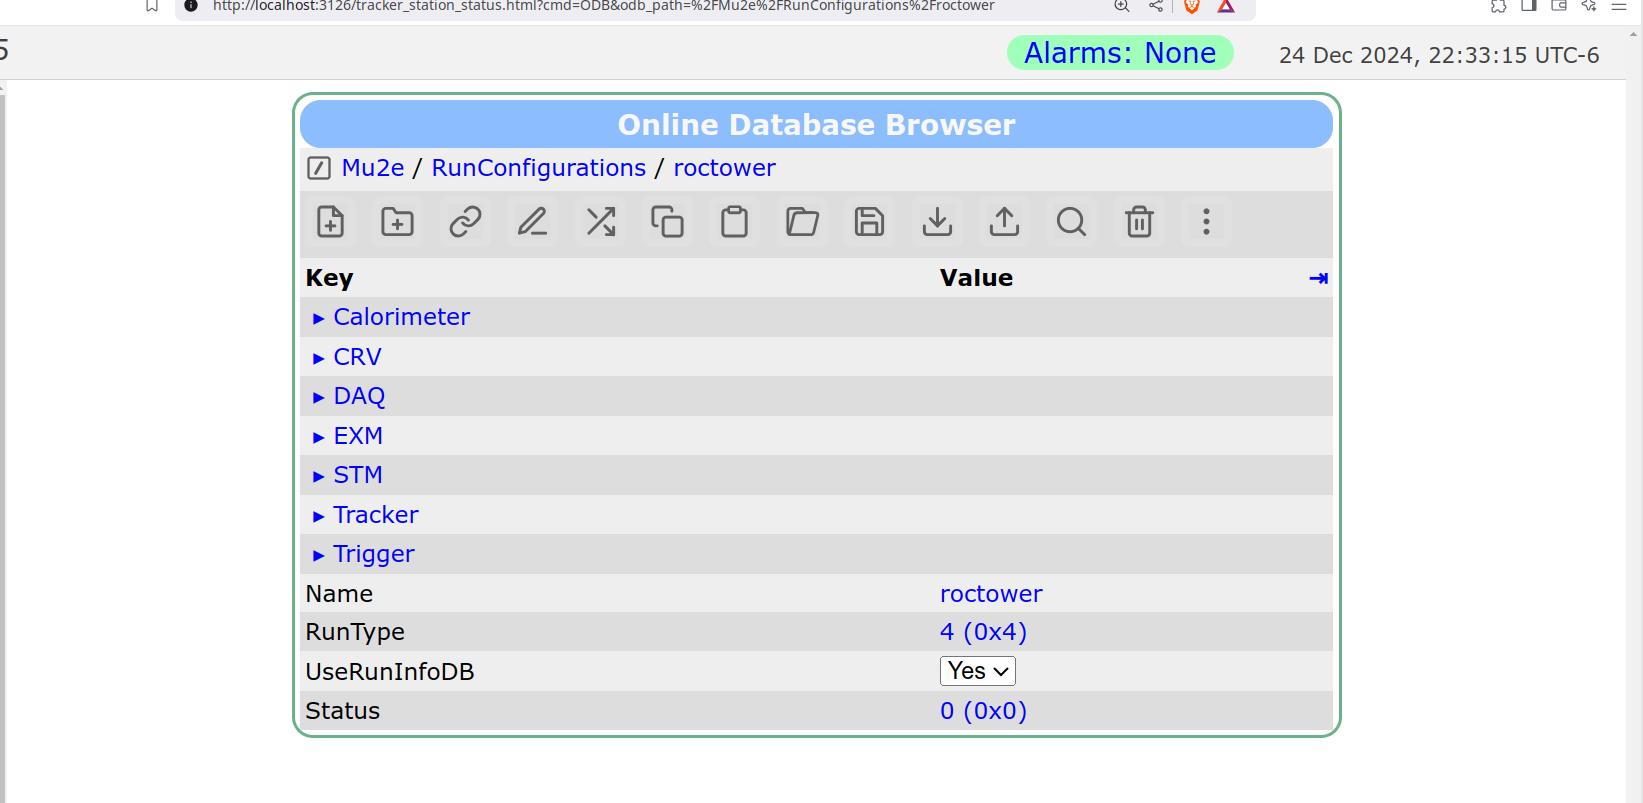
\includegraphics[width=0.95\textwidth]{png/configuration_top}
      }
    };
    % \node [text width=8cm, scale=1.0] at (14.5,0.5) {$\mu_B$, expected background mean};
    % \node [text width=8cm, scale=1.0, rotate={90}] at (1.5,7.5) { $S_{D}$, ``discovery'' signal strength  };
  \end{tikzpicture}
  \caption{
    \label{figure:configuration_top}
    Top view of the configuration called 'roctower' - a 6-ROC tracker test stand in IERC
  }
\end{figure}

%%%%%%%%%%%%%%%%%%%%%%%%%%%%%%%%%%%%%%%%%%%%%%%%%%%%%%%%%%%%%%%%%%%%%%%%%%%%%%
\subsection{Data Model}

* configuration  : first step                                                
- request run number
- set "CONFIGURE" in /Mu2e/Commands/ (this could be done via the Sequencer)

- a configuration frontend (python)
  - identifies enabled subdetectors
  - passses the command to the enabled subdetector configuration frontends (python)
  - the subsystem configuration frontends are completely independent
  - waits for some time for them to act
  - subssytem configuration frontends complete, set Status and 
  - after the configuration succeeds or the time expires, the configuration
    frontend forces stop of its execution
  - it sets the command execution status and returns to MIDAS

- if the configuration step has completed successfully, a new run is started

- each subsystem has Enabled and Status attributed in ODB
- to exclude the failed sysbystem from the configuration: set Enabled=0

- DAQ configuration:

  - CFO configuration
  - configuration of each node

  - per node:

    - one or two boardreaders
    - event builder
    - data logger
    - dispatcher

    - each of them has Enabled attribute

  - TFM talks to ODB , identifies enabled processes and submits jobs only
    for them

  - there is a "Generate FCL" command which generates FCLs
    for an given? active? configuration

- as the DAQ configuration depends on the enabled detector configuration,
  the DAQ is configured afer all subdetectors 


* monitoring of the detector status                                          

- each subdetector has "Enabled" and "Status" parameters
\begin{verbatim}
|--------+-----------+--------------------------------------------|
| status | color     | meaning                                    |
|--------+-----------+--------------------------------------------|
|     -2 | dark gray | Enabled=0                                  |
|     -1 | gray      | enabled=1, but no initialization performed |
|      0 | red       | enabled=1, failed initialization           |
|      1 | green     | enabled=1, initialized OK                  |
|--------+-----------+--------------------------------------------|
\end{verbatim}

* description in ODB                                                         
- no links across configuration boundaries
- links allowed within the configuration , i.e.
  - DTC --> tracker panel
  - boardreader DTC --> DTC configuration
- ActiveConfiguration
* commands and execution
 a command has three fields
 
1) Run     : 0: "no request to run"  1: "requested to run" 
2) Status  : int
   < 0: "execution failed" , the value gives the error code
   0  : "execution finished OK"
   1  : "execution in progress"

   after the Status is set, the same client resets Run=0
3) Parameters :


%%%%%%%%%%%%%%%%%%%%%%%%%%%%%%%%%%%%%%%%%%%%%%%%%%%%%%%%%%%%%%%%%%%%%%%%%%%%%%
\subsection{DAQ-specific frontends}

\begin{itemize}
\item
  one monitoring/control frontend per DAQ server. Monitoring:
  \begin{itemize}
  \item
    2 DTC's with 6 ROCs per DTC
  \item
    ARTDAQ processes:
    \begin{itemize}
    \item
      2 boardreaders, N event builders, potentially a data logger, and a dispatcher
    \end{itemize}
  \item
    overall health: amount of free space available
  \end{itemize}
\item
  emulated CFO:
  \begin{itemize}
  \item
    currently : a separate frontend 
  \item 
    make the CFO frontend a separate thread of the node frontend
  \end{itemize}
\item
  external CFO frontend 
\item
  global control frontend:
\end{itemize}

%%%%%%%%%%%%%%%%%%%%%%%%%%%%%%%%%%%%%%%%%%%%%%%%%%%%%%%%%%%%%%%%%%%%%%%%%%%%%%
\subsection{Run transition sequence}

This section describes the sequence in which different run transitions
are executed by the system components.

\add{does OTSDAQ allow different execution sequences for
  different run transitions ? }

%%%%%%%%%%%%%%%%%%%%%%%%%%%%%%%%%%%%%%%%%%%%%%%%%%%%%%%%%%%%%%%%%%%%%%%%%%%%%%
\subsubsection{Begin Run}
\begin{itemize}
\item
  subdetector hardware configuration
\item
  sequencer requests the new run
\item
  MIDAS begin start
  \begin{itemize}
  \item
    global config frontend - pre-begin run records the transition start
  \item
    DTC configuration frontends 
  \item
    TFM frontend - artdaq processes
  \item
    CFO frontend 
  \item
    global configuration frontend
  \end{itemize}
\end{itemize}

%%%%%%%%%%%%%%%%%%%%%%%%%%%%%%%%%%%%%%%%%%%%%%%%%%%%%%%%%%%%%%%%%%%%%%%%%%%%%%
\subsubsection{End Run}
\begin{itemize}
\item
  MIDAS end start
  \begin{itemize}
  \item
    global configuration frontend pre-end run callback: records
    the transition start
  \item
    CFO frontend stops executing the run plan
  \item
    TFM frontend - artdaq processes
  \item
    DTC frontends - artdaq processes
  \item
    global configuration frontend records the end of transition
  \end{itemize}
\end{itemize}


%%%%%%%%%%%%%%%%%%%%%%%%%%%%%%%%%%%%%%%%%%%%%%%%%%%%%%%%%%%%%%%%%%%%%%%%%%%%%%
\subsubsection{Pause and Resume Run}

Pause the run:

\begin{itemize}
\item
  configuration frontend: pre-transition callback: record the transition start
\item
  CFO frontend: disable output 
\item
  TFM frontend: pause the run
\item
  DTC frontends: do nothing 
\item
  configuration frontend: record the transition end
\end{itemize}

%%%%%%%%%%%%%%%%%%%%%%%%%%%%%%%%%%%%%%%%%%%%%%%%%%%%%%%%%%%%%%%%%%%%%%%%%%%%%%
\subsubsection{Resume Run}

Pause the run:

\begin{itemize}
\item
  configuration frontend: pre-transition callback: record the transition start
\item
  TFM frontend: pause the run
\item
  DTC frontends: do nothing 
\item
  CFO frontend: enable output 
\item
  configuration frontend: record the transition end
\end{itemize}


%%% Local Variables:
%%% mode: latex
%%% TeX-master: t
%%% End:
